\documentclass[12pt,Letter]{article}
%\usepackage[margin=3cm]{geometry}
\usepackage{listings}
\usepackage{graphicx}
\usepackage{float}
\usepackage{color}
\usepackage{tabularx}
\usepackage{adjustbox}
%\usepackage{tikz}
\usepackage[justification=centering]{caption}
%\usetikzlibrary{shapes.geometric,arrows}
%\renewcommand{\lstlistingname}{\textbf{Program}}
\newcommand{\sanper}{\textsc{sanper-1 elu}}
%setting up flowcharts
%\tikzstyle{startstop} = [rectangle, rounded corners, minimum width=3cm, minimum height = 1cm, text centered, draw=black, fill=red!30]

%\tikzstyle{process} = [rectangle, minimum width=3cm, minimum height = 1cm, text centered, text width = 3cm, draw=black, fill=orange!30]

%\tikzstyle{decision} = [diamond,  minimum width=1cm, minimum height = .5cm, text centered, text width = 2cm, draw=black, fill=green!30]

%\tikzstyle{arrow} = [thick, ->,>=stealth]

\definecolor{mygreen}{rgb}{0,0.6,0}
\definecolor{mygray}{rgb}{0.5,0.5,0.5}
\definecolor{mymauve}{rgb}{0.58,0,0.82}

\lstset{ %
	backgroundcolor=\color{white},   % choose the background color; you must add \usepackage{color} or \usepackage{xcolor}
	basicstyle=\footnotesize,        % the size of the fonts that are used for the code
	breakatwhitespace=false,         % sets if automatic breaks should only happen at whitespace
	breaklines=true,                 % sets automatic line breaking
	captionpos=b,                    % sets the caption-position to bottom
	commentstyle=\color{mygreen},    % comment style
	deletekeywords={...},            % if you want to delete keywords from the given language
	escapeinside={\%*}{*)},          % if you want to add LaTeX within your code
	extendedchars=true,              % lets you use non-ASCII characters; for 8-bits encodings only, does not work with UTF-8
%	frame=single,                    % adds a frame around the code
	keepspaces=true,                 % keeps spaces in text, useful for keeping indentation of code (possibly needs columns=flexible)
	keywordstyle=\color{blue},       % keyword style
	language=[Motorola68k]Assembler, % the language of the code
	morekeywords={*,...},            % if you want to add more keywords to the set
	numbers=left,                    % where to put the line-numbers; possible values are (none, left, right)
	numbersep=5pt,                   % how far the line-numbers are from the code
	numberstyle=\small\color{mygray}, % the style that is used for the line-numbers
	rulecolor=\color{black},         % if not set, the frame-color may be changed on line-breaks within not-black text (e.g. comments (green here))
	showspaces=false,                % show spaces everywhere adding particular underscores; it overrides 'showstringspaces'
	showstringspaces=false,          % underline spaces within strings only
	showtabs=false,                  % show tabs within strings adding particular underscores
	stepnumber=1,                    % step between two line-numbers. If it's 1, each line will be numbered
	stringstyle=\color{mymauve},     % string literal style
	tabsize=2                  % sets default tabsize to 2 spac                  % show the filename of files included with \lstinputlisting; also try caption instead of title
}

\begin{document}

\begin{titlepage}
	\begin{center}
		
		
		% Upper part of the page. The '~' is needed because \\
		% only works if a paragraph has started.
		\vfill
		
		\textsc{\LARGE Experiment 6: Input/Output Design}\\[1.5cm]
		
		\Large Adam Sumner\\[0.5cm]
		
		\Large Illinois Institute of Technology\\[0.5cm]
		
		\Large ECE 441-01\\[0.5cm]	
		% Author and supervisor
		\noindent
		\vfill
		\large \textbf{Lab Date:} March 31st, 2015\hfill
		\large \textbf{Due Date:} April 14th, 2015
		% Bottom of the page
		
		
	\end{center}
\end{titlepage}

\section{Introduction}
The purpose of this experiment is to introduce the student to the concepts of memory mapped I/O interrupts. The student will design and implement hardware and software to read data from a DIP switch, pass the data to a software counter, and display the counter's outputs on two 7-Segment displays.
\section{Background}
\subsection{Memory-Mapped Input/Output(I/O)}
There are two different types of philosophies when it comes to interfacing to I/O devices. These are known as ``Memory Mapped" I/O and ``Isolated" I/O. The MC68000 uses the memory-mapped I/O philosophy. This implies that all I/O devices are accessed by reading and writing to memory locations within the microprocessor's address space\cite{expman}.
\subsection{Interrupts}
The MC68000 microprocessor is equipped with 3 interrupt request signals ($\overline{IPL2}$, $\overline{IPL1}$, and $\overline{IPL0}$) which provide a maximum of 7 distinct interrupt levels, and a normal operating level (Level 0). The status Register contains three Interrupt Mask Bits (I2,I1, and I0) which are the logical complement of the interrupt hardware signals. Table \ref{tab:mask} illustrates the relationship between the interrupt request signals and the interrupt mask bits\cite{expman}.

\begin{table}[H]
	\noindent\adjustbox{max width=\textwidth}{
	\begin{tabular}{c c c | c c c | c}
		 $\overline{IPL2}$ &  $\overline{IPL1}$ & $\overline{IPL0}$ &  I2 &  I1 & I0 & Requested Interrupt Level
		 \\ \hline
		 0 & 0 & 0 & 1 & 1 & 1 & 7\\
		 0 & 0 & 1 & 1 & 1 & 0 & 6\\
		 0 & 1 & 0 & 1 & 0 & 1 & 5 \\
		 0 & 1 & 1 & 1 & 0 & 0 & 4 \\
		 1 & 0 & 0 & 0 & 1 & 1 & 3 \\
		 1 & 0 & 1 & 0 & 1 & 0 & 2 \\
		 1 & 1 & 0 & 0 & 0 & 1 & 1\\
		 1 & 1 & 1 & 0 & 0 & 0 & 0(none)
	\end{tabular}
	}
	\caption{Interrupt Request/Mask Relationship}
	\label{tab:mask}
\end{table}

\noindent When dealing with interrupts, the device requesting service activates a hardware signal called an Interrupt Request line $\overline{IRQ}$. The $\overline{IRQ}$ from several peripheral devices are prioritized, encoded , and inputted to the three interrupt request lines of the MC68000. They are made pending until the CPU completes the current instruction being executed. Once completed, the current state is saved on stack, and an interrupt acknowledge cycle begins. The MC68000 compares the incoming interrupt request to the current interrupt priority level in the Status Register. If the level is less than or equal to the current interrupt priority level, the interrupt is not serviced. Table \ref{tab:sanper} shows the list of interrupt level settings for the \sanper \cite{expman}.

\begin{table}[H]
	\noindent\adjustbox{max width=\textwidth}{
		\begin{tabular}{c c c}
			\underline{Interrupt Level} & \underline{Interrupting Device} & \underline{Vector No. (Decimal)} \\
			7 & ABORT Switch & 31 \\
			6 & ACIA2 (Host Port) & 30\\
			5 & ACIA1 (Terminal Port) & 29 \\
			4 & ACIA3, Speech, PIA & 28 \\
			3 & PI/T Parallel Ports  $\overline{PIRQ}$ & U.V \\
			2 & PI/T Timer $(\overline{TOUT})$ & U.V \\
			1 & System Expansion Board & A.V or U.V \\
			0 & Normal CPU Operation & Not Used
		\end{tabular}

	}

	\vspace{0.5cm}
	Where:	\hspace{3.5ex}U.V. = User-vectored interrupt\\
	\-\ \hspace{11ex}A.V. = Auto-vectored interrupt
	\caption{Sanper Interrupt Signals}
	\label{tab:sanper}
\end{table}

\noindent $\overline{IRQ1}$ is accessible to the user through the System Expansion Board and can be assumed to have been configured for Auto-Vectored Interrupts on Level 1.
\section{Equipment/Procedure}
\subsection{Equipment}
\begin{itemize}
	\item \textsc{SANPER-1 Educational Lab Unit}
	\item Computer with TUTOR software
	\item DIP Switch
	\item 1K Pull up resistors
	\item 7-Segment Display
	\item Octal Transparent Latch with 3-State Outputs
	\item Inverter Chip
	\item Open Collector Inverter Chip
	\item NOR Gate Chip
	\item NAND Gate Chip

\end{itemize}
\subsection{Procedure}
The student is to design and draw a detailed schematic of the hardware required to perform the input functionality of reading from a DIP Switch, and the output functionality of writing to two 7-Segment displays. Once finished, the student is to implement the schematic on a breadboard, and connect the hardware to the \sanper. After this, the student must write an interrupt service routine that performs the input functionality of reading data from the DIP Switch, and performs the output functionality of writing to the two 7-Segment Displays.
\section{Results}
Section \ref{sec:hardware} shows the circuit schematic while this Section shows the physical implementation of the circuit. The results obtained correctly matched up with the expected result and the LED I/O timer was successfully implemented.
\begin{figure}
\centering
\includegraphics[width=1\linewidth]{20150407_111232}
\caption{Full Circuit View}
\label{fig:20150407_111232}
\end{figure}
\begin{figure}
\centering
\includegraphics[width=1\linewidth]{20150407_105931}
\caption{Connected to Sanper Unit}
\label{fig:20150407_105931}
\end{figure}

\begin{figure}[H]
\centering
\includegraphics[width=1\linewidth]{20150407_105924}
\caption{Close Up of LEDs}
\label{fig:closeup}
\end{figure}

\section{Discussion}
\subsection{Answers to Discussion Problems}
\begin{enumerate}
	\item Program can be found in Section \ref{sec:memtest}
	\item Schematic can be found in Section \ref{sec:hardware}
	\item Figure 8-3(Sheet 2) from the Motorola Educational Computer Board User's Manual has an error and doesn't show the ABORT circuitry so I'll discuss how I would design the circuitry instead. I'd wire the button into an encoder connected to the IRQ lines. When the button is pressed, it'll encode a 7 or 111b. Interrupt number 7 is unmaskable, so it would ensure that the system would break out of the executing program. The ABORT button works by ensuring the vector generated by the interrupt level 7 points to a program that can recover back into the TUTOR software.
	\item If the CPU sends an interrupt acknowledge after receiving an interrupt request, but no device responds to the acknowledge, a spurious interrupt is generated. It prevents the CPU from waiting forever for an external device to respond. An uninitialized interrupt is generated when a peripheral hasn't been configured yet, but it generates an interrupt. Peripherals designed for 68000 based systems automatically supply the uninitialized vector 0x0F.
	\item Auto-Vectored Interrupts are associated with peripherals designed for 8-bit processors. This is because 8-bit processors cannot provide a vector during an IACK cycle. There are 7 Auto-Vectored Interrupts. The User-Vector interrupt is intended for peripherals that can provide an 8-bit vector number. There are 256 Auto-Vector Interrupts.
	\item IACK Cycle:
		\begin{enumerate}
			\item The peripheral signals on its interrupt line
			\item The line is encoded into an interrupt level
			\item The CPU completes the current instruction then saves
			its current state onto the stack
			\item The level is checked against the SR
			\item If the incoming level is higher than the current level, the interrupt is serviced
			\item If it's less than or equal to the current level, the interrupt is not serviced
		\end{enumerate}
\end{enumerate}
\section{Conclusion} 
Overall the experiment was a success. The student was adequately introduced to the concepts of memory mapped I/O interrupts. The I/O hardware design was successfully implemented and tested. Subsequently, the code that enabled the I/O functionality of a DIP switch was also successfully implemented and tested. Further testing of the \sanper's I/O capability can be conducted by accepting input of more than 8 bits.
\begin{thebibliography}{1}
	\bibitem{expman} Experiment 6 Lab Manual
	\bibitem{ecbm} Educational Computer Board Manual
	\bibitem{m68k}MC68K User Manual
	\bibitem{sanper}SANPER-1 ELU User Manual
	
	
\end{thebibliography}
  

\section{Appendix}
\label{appendix}
\subsection{Code}\label{code}
\subsubsection{LED Counter}\label{sec:memtest}
\lstinputlisting{prog.X68}
\subsection{Hardware}\label{sec:hardware}
\begin{figure}[H]
\centering
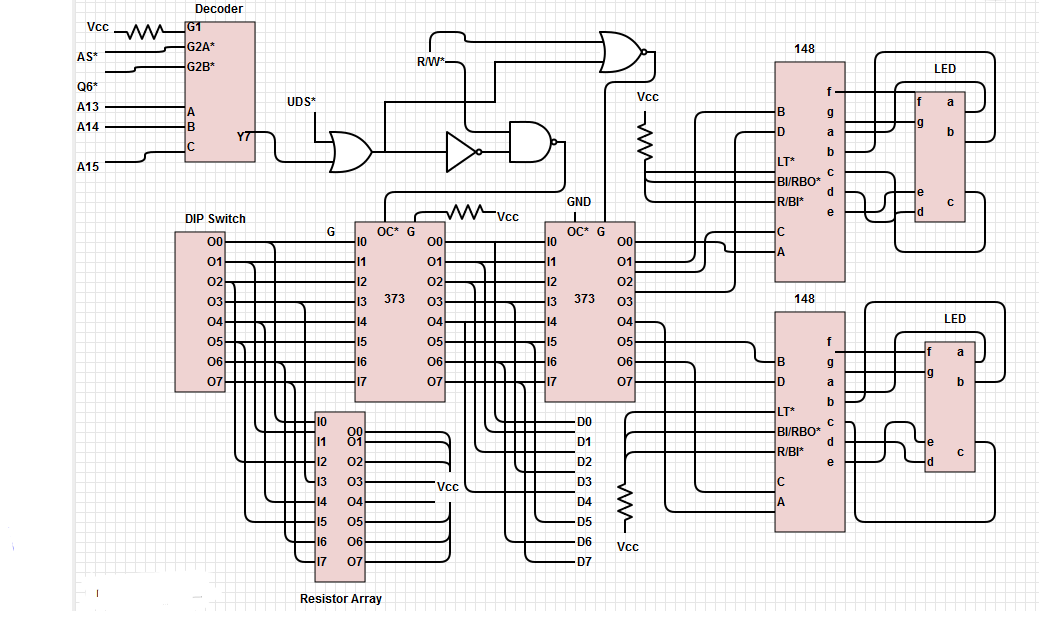
\includegraphics[width=1\linewidth]{lab6schematic}
\caption{I/O Hardware Schematic}
\label{fig:lab6schematic}
\end{figure}

\end{document}